\section{Fast project}

\subsection{Project of the \texttt{Bluetooth} communications}

As said in the fast analysis, \texttt{Bluetooth} is the chosen communication technology to realize the interaction between robot and user's device.
Android developer documentation fully explain how to set up \href{https://developer.android.com/guide/topics/connectivity/bluetooth}{\texttt{Bluetooth}} while \href{https://github.com/LM-96/MobileSystemProject/tree/main/kBluez}{\texttt{kBluez}} is made by us to make this project work.

About \texttt{Android}, as suggested by the documentation, the main operation to \textit{connect} to a device is:
\begin{itemize}
	\item \textbf{find} the device by executing a \textit{discovery} operation;
	\item \textbf{connect} to the discovered device obtaining a \href{https://developer.android.com/reference/android/bluetooth/BluetoothSocket}{\texttt{BluetoothSocket}};
	\item \textbf{exchange} data throw the socket.
\end{itemize}
\textbf{Notice that differently from the normal \textit{INET} socket, the \texttt{Bluetooth} connection can be established only using the \texttt{UUID} of a \href{https://en.wikipedia.org/wiki/List_of_Bluetooth_protocols\#Radio_frequency_communication_(RFCOMM)}{\texttt{RFCOMM}} service}.

In addition to this, in \texttt{Android} some operations are natively realized with some asynchronous mechanism such as \href{https://developer.android.com/reference/android/content/IntentFilter}{\texttt{IntentFilter}} or \href{https://developer.android.com/reference/android/content/BroadcastReceiver}{\texttt{BroadcastReceiver}}. The obvious motivation for that is to prevent some \textit{unconscious} use of blocking \texttt{IO} operations on the main thread that with this mechanism is avoided.

Even if this way \textit{to do the things} should more safe, it introduces some complications especially for the legibility of code: indeed the developer must register \textit{receiver} that will be activated when required the action has been performed, like imposed by \texttt{Intent} or \texttt{BroadcastReceiver}.

Then, consider if you want to perform a discovery operation using bluetooth in order to search for devices, storing the results in a collection. Following the android guide, the developer must use this pattern:

\begin{lstlisting}[language=Kotlin]
//The collection to store results
val devices = ConcurrentLinkedDeque<BluetoothDevice>()
	
override fun onCreate(savedInstanceState: Bundle?) {
	...
	
	// Register for broadcasts when a device is discovered.
	val filter = IntentFilter(BluetoothDevice.ACTION_FOUND)
	registerReceiver(receiver, filter)
	
	//Start the discovery
	bluetoothAdapter.startDiscovery()
}

// Create a BroadcastReceiver for ACTION_FOUND.
private val receiver = object : BroadcastReceiver() {
	
	override fun onReceive(context: Context, intent: Intent) {
		val action: String = intent.action
		when(action) {
			BluetoothDevice.ACTION_FOUND -> {
				// Discovery has found a device. Get the BluetoothDevice
				// object and its info from the Intent.
				val device: BluetoothDevice =
				intent.getParcelableExtra(BluetoothDevice.EXTRA_DEVICE)
				devices.add(device)
			}
		}
	}
}

override fun onDestroy() {
	super.onDestroy()
	...
	
	// Don't forget to unregister the ACTION_FOUND receiver.
	unregisterReceiver(receiver)
}
\end{lstlisting}

We could make this code more \textit{elegant} using the smart notation of \texttt{Kotlin} lambdas, but however asynchronism could confuse the developer. In addition to this, if the operation are nested (for example, \textit{if a device is found that connect to it}) then code inevitably ends with a \textit{storm} of lambdas which can be very illegible.

For this reason, we decide to provide a solution that restore the synchronism by using the simple class \href{https://github.com/LucaLand/MobileSystemsProject-LL/blob/0.9.1/app/src/main/java/it/unibo/mobilesystems/bluetooth/BluetoothDiscoveryBroadcastReceiver.kt}{\texttt{BluetoothDiscoveryBroadcastReceiver}} and coroutines:
\begin{lstlisting}[language=Kotlin]
private val resultChan = Channel<Any>()
private val bluetoothDiscoveryBroadcastReceiver =
						BluetoothDiscoveryBroadcastReceiver()
private val controllerOnDeviceDiscovered : (BluetoothDevice) -> Unit =
{ device ->
	scope.launch {resultChan.send(device)}
}
private val controllerOnDiscoveryFinished : () -> Unit =
{
	scope.launch {resultChan.send(BluetoothAdapter.ACTION_DISCOVERY_FINISHED)}
}
	
suspend fun discoverDevice(activity : Activity,
							onDeviceDiscovered : (BluetoothDevice) -> Unit = {}) :
									Set<BluetoothDevice> {
	bluetoothDiscoveryBroadcastReceiver
				.addOnDeviceDiscovered(onDeviceDiscovered)
	bluetoothDiscoveryBroadcastReceiver
				.addOnDeviceDiscovered(controllerOnDeviceDiscovered)
	bluetoothDiscoveryBroadcastReceiver
				.addOnDiscoveryFinished(controllerOnDiscoveryFinished)
	
	withContext(Dispatchers.Main) {
		val actionFoundFilter = IntentFilter(BluetoothDevice.ACTION_FOUND)
		activity.registerReceiver(bluetoothDiscoveryBroadcastReceiver,
									actionFoundFilter)
		val discoveryFinishedFilter = IntentFilter(
								BluetoothAdapter.ACTION_DISCOVERY_FINISHED)
		activity.registerReceiver(bluetoothDiscoveryBroadcastReceiver,
									discoveryFinishedFilter)
		bluetoothAdapter!!.startDiscovery()
	}

	val devices = mutableSetOf<BluetoothDevice>()
	var res : Any
	do {
		res = resultChan.receive()
		when(res) {
			is BluetoothDevice -> {
				devices.add(res)
			}
		}
	} while (!(res is String &&
					res == BluetoothAdapter.ACTION_DISCOVERY_FINISHED))

	withContext(Dispatchers.Main) {
		activity.unregisterReceiver(bluetoothDiscoveryBroadcastReceiver)
	}
	bluetoothDiscoveryBroadcastReceiver
				.removeOnDeviceDiscovered(onDeviceDiscovered)
	bluetoothDiscoveryBroadcastReceiver
				.removeOnDeviceDiscovered(controllerOnDeviceDiscovered)
	bluetoothDiscoveryBroadcastReceiver
				.removeOnDiscoveryFinished(controllerOnDiscoveryFinished)

	return devices
}
\end{lstlisting}

\textbf{Notice thatn\texttt{discoverDevice} is a method that is executed by a coroutine that waits for the discovery operation completion.} Theoretically, this method should introduce only a very small overhead caused by the \texttt{scope.launch} that is present by the lambda that are invoked from the \texttt{BroadcastReceiver} of the bluetooth. Indeed, the suspension of calling coroutine on the result channel should introduce no additional costs.

In future implementations, this function might be refined in order to be called also from coroutines that are executing on the main thread by using the appropriate dispatcher.

\begin{figure}[h!]
	\centering
	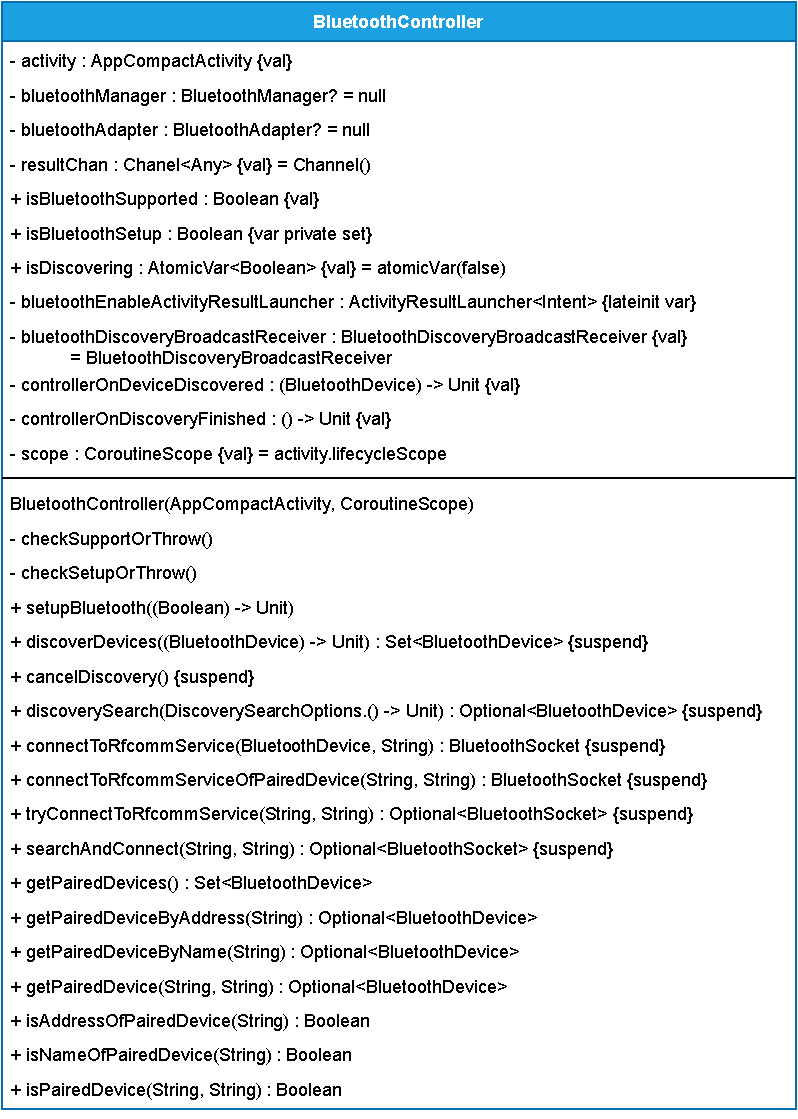
\includegraphics[width=0.7\textwidth]{img/bluetoothcontroller_uml.pdf}
	\caption{UML diagram of \texttt{BluetoothController}}
	\label{fig:bluetoothcontroller_uml}
\end{figure}

Other Bluetooth operations also use this pattern so the figure \ref{fig:bluetoothcontroller_uml} shows the \texttt{UML} diagram of a \textit{controller} for the Bluetooth that can be used from \texttt{BluetoothActivity}.

\begin{figure}[h!]
	\centering
	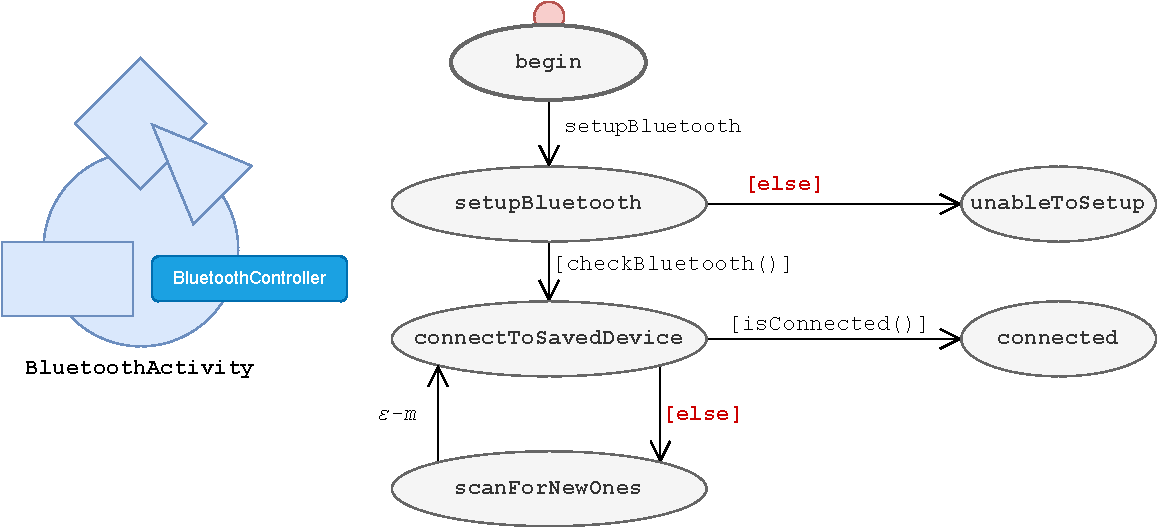
\includegraphics[width=\textwidth]{img/bluetoothactivity.pdf}
	\caption{State diagram of \texttt{BluetoothActivity}}
	\label{fig:bluetoothactivity}
\end{figure}

The figure \ref{fig:bluetoothactivity} shows the state diagram of the \href{https://github.com/LucaLand/MobileSystemsProject-LL/blob/0.9.1/app/src/main/java/it/unibo/mobilesystems/BluetoothConnectionActivity.kt}{\texttt{BluetoothActivity}}. Notice that \textbf{the method \texttt{setupBluetooth} of the controller must be called into the \texttt{onCreate} method of \texttt{Activity} in order to make it work}.

About the states in \texttt{BluetoothActivity}:
\begin{itemize}
	\item \textbf{begin}:\\
	in this state the actor prepare itself for doing the Bluetooth operations and showing results.
	
	\item \textbf{setupBluetooth}:\\
	the actor check if Bluetooth is already been set up by the activity: if not, the actor goes into \textbf{unableToSetupStatus} that only shows to the user a toast saying that it is not possible to use Bluetooth.
	
	\item \textbf{connectToSavedDevice}:\\
	the actor tries to connect the \textit{saved device} that is the last correctly used by the application.
	
	\item \textbf{scanForNewOnes}:\\
	the actor uses the controller to scan for devices showing the found in real time. When the user selects a device, the actor immediately transit to \textbf{connectToSavedDevice} by epsilon move.
	
\end{itemize}
\textbf{We also underline that the actor waits for a \texttt{setupBluetooth} message from its activity in order to perform Bluetooth operations}: this allows to set up Bluetooth from the \texttt{onCreate}, notifying the actor when this operation is concluded, so the actor can correctly use a well initiated controller. 